\documentclass[12pt,letterpaper]{article}

\newenvironment{proof}{\noindent{\bf Proof:}}{\qed\bigskip}

\newtheorem{theorem}{Theorem}
\newtheorem{corollary}{Corollary}
\newtheorem{lemma}{Lemma} 
\newtheorem{claim}{Claim}
\newtheorem{fact}{Fact}
\newtheorem{definition}{Definition}
\newtheorem{assumption}{Assumption}
\newtheorem{observation}{Observation}
\newtheorem{example}{Example}
\newcommand{\qed}{\rule{7pt}{7pt}}

\newcommand{\assignment}[4]{
	\thispagestyle{plain} 
	\newpage
	\setcounter{page}{1}
	\noindent
	\begin{center}
		\framebox{ \vbox{ \hbox to 6.28in
				{\bf CS412: Introduction to Data Mining \hfill #1}
				\vspace{4mm}
				\hbox to 6.28in
				{\hspace{2.5in}\large\mbox{Problem Set #2}}
				\vspace{4mm}
				\hbox to 6.28in
				{{\it Handed Out: #3 \hfill Due: #4}}
			}}
		\end{center}
	}
	
	\newcommand{\solution}[4]{
		\thispagestyle{plain} 
		\newpage
		\setcounter{page}{1}
		\noindent
		\begin{center}
			\framebox{ \vbox{ \hbox to 6.28in
					{\bf CS412:   Introduction to Data Mining \hfill #4}
					\vspace{4mm}
					\hbox to 6.28in
					{\hspace{2.5in}\large\mbox{#3}}
					\vspace{4mm}
					\hbox to 6.28in
					{#1 \hfill {\it #2}}
				}}
			\end{center}
			\markright{#1}
		}
		
		\newenvironment{algorithm}
		{\begin{center}
				\begin{tabular}{|l|}
					\hline
					\begin{minipage}{1in}
						\begin{tabbing}
							\quad\=\qquad\=\qquad\=\qquad\=\qquad\=\qquad\=\qquad\=\kill}
						{\end{tabbing}
					\end{minipage} \\
					\hline
				\end{tabular}
			\end{center}}
			
			\def\Comment#1{\textsf{\textsl{$\langle\!\langle$#1\/$\rangle\!\rangle$}}}
			
			
			%\documentclass{article}
			\usepackage{multirow}
			\usepackage{amsmath}
			\usepackage{amssymb}
			\usepackage{algorithm}
			\usepackage{algpseudocode}
			\setlength{\parindent}{0pt}
			\usepackage{graphicx}
			\usepackage{ctable}
			%\usepackage{fullpage}
			%\usepackage{setspace} 
			\usepackage{float}
			%\usepackage{listings} 
			%\usepackage{bbm}
			\usepackage{bigstrut}
			%\usepackage{caption}
			%\usepackage{subcaption}
			%\usepackage{algpseudocode}
			%\usepackage{algorithm}
			\usepackage{epstopdf}
			
			\usepackage{listings}
			\usepackage{color}
			\usepackage[utf8]{inputenc}
			
			\definecolor{dkgreen}{rgb}{0,0.6,0}
			\definecolor{gray}{rgb}{0.5,0.5,0.5}
			\definecolor{mauve}{rgb}{0.58,0,0.82}
			
			\lstset{frame=tb,
				language=matlab,
				aboveskip=3mm,
				belowskip=3mm,
				showstringspaces=false,
				columns=flexible,
				basicstyle={\small\ttfamily},
				numbers=none,
				numberstyle=\tiny\color{gray},
				keywordstyle=\color{blue},
				commentstyle=\color{dkgreen},
				stringstyle=\color{mauve},
				breaklines=true,
				breakatwhitespace=true,
				tabsize=3
			}
			
			
			\oddsidemargin 0in
			\evensidemargin 0in
			\textwidth 6.5in
			\topmargin -0.5in
			\textheight 9.0in
			\usepackage{multirow}
			\usepackage{hyperref}
			
			\hypersetup{colorlinks=true}
			\usepackage{color}
			
			\newenvironment{ans}{%
				\vspace{5mm}
				\textcolor{red}{{\sf Answer}}\\%
			}
			{%
			}
			
			\begin{document}
				
				
				\solution{Li Miao}{Due: 11/19/2015 11:59pm}{Assignment 4}{Fall 2015}
				% Fill in the above, for example, as follows:
				% \solution{Joe Smith}{\today}{1}{Fall 2012}
				
				\pagestyle{myheadings}  % Leave this command alone
				
		
				
				\section{Constraint pattern mining (5 points)}
				For the following constraints, write down your answer if they are (strongly convertible, convertible) Anti-monotone, Monotone or Succinct. 
				
				\textbf{Purpose} 
				\begin{itemize}\vspace{-2mm}\setlength\itemsep{-1mm}
					\item Have a better understanding of constraint pattern mining.
				\end{itemize}
				\textbf{Requirements}
				\begin{itemize}\vspace{-2mm}\setlength\itemsep{-1mm}
					\item A short explanation to justify if the constraint belongs to \textbf{EACH} type is required. To show a constraint is not of one type, use a simple example.
				\end{itemize}
				
				\begin{itemize}
					\item[a.] (1', L1) for a set of values $S$, and a value $v$, constraint $v \in S$
					\item[b.] (1', L1) for a set of values $S$, and a value $v$, constraint $max(S) \geq v$
					\item[c.] (1', L1) for a set of values $S$, and a value $v$, constraint $max(S) \leq v$
					\item[d.] (2', L2) for a set of values $S$, and a value $v$, constraints $avg(S) \geq v$ and $avg(S) \leq v$
				\end{itemize}
				
				
				
				\section{Advanced pattern mining (10 points)}
				For each question below, indicate if the statement is \textbf{true} or \textbf{false}.\\
				
				\textbf{Purpose} 
				\begin{itemize}\vspace{-2mm}\setlength\itemsep{-1mm}
					\item Have a better understanding of advanced pattern mining.
				\end{itemize}
				\textbf{Requirements}
				\begin{itemize}\vspace{-2mm}\setlength\itemsep{-1mm}
					\item For each sub-question, select \textbf{true (T)} or \textbf{false (F)} and also write down a brief explanation. You will \textbf{NOT} get credit without an explanation. 
				\end{itemize}
				\begin{itemize}
					\item[a.] (2', L2) \textbf{T/F.}  Convertible constraint porperty cannot be exploited in an Apriori-based mining algorithm.
					\item[b.] (2', L2) \textbf{T/F.}  In \textit{PrefixSpan}, physical project is not used because of its slow performance.
					\item[c.] (2', L1) \textbf{T/F.}  Mining closed frequent graphs only is lossless compression of the graph database.
					\item[d.] (2', L3) \textbf{T/F.}  In sequential pattern mining, the number of length-2 candidates generated from $x$ frequent length-1 patterns is $\frac{3}{2}x^2 - \frac{1}{2}x$
					\item[e.] (2', L3) \textbf{T/F.}  For nontrivial constraints (trivial constraints are those that are satisfied by every possible pattern), it cannot be monotone and anti-monotone at the same time.
				\end{itemize}
				
				
				
				\section{Sequential pattern mining (20 points)}
				Use a toy dataset to perform sequential pattern mining algorithms.
				
				\textbf{Purpose} 
				\begin{itemize}\vspace{-2mm}\setlength\itemsep{-1mm}
					\item Work on sequential pattern mining using \textit{GSP} and \textit{PrefixSpan}
				\end{itemize}
				\textbf{Requirements}
				\begin{itemize}\vspace{-2mm}\setlength\itemsep{-1mm}
					\item Write down each step as detail as possible.
				\end{itemize}
				
				Suppose a toy sequence database $D$ contains three sequences as follows. Let the minimum support be 3.
				
				\begin{tabular}{c|l}
					% after \\: \hline or \cline{col1-col2} \cline{col3-col4} ...
					customer\_id & shopping sequence \\\hline
					1 & $(bc) (de) f$ \\
					2 & $ bc d ef$ \\
					3 & $(bc) d b e g f$ \\\hline
				\end{tabular}\\
				
				The following questions require you to perform GSP algorithm.
				
				\begin{enumerate}
					\item [(1)] (2', L2) Scan database once, list length-1 sequential pattern candidates $C_1$ and the result $L_1$ after pruning. 
					\item [(2)] (3', L2) Following, generate $C_2$, and $L_2$. \textit{Hint: do not miss any candidates in $C_2$}
					\item [(3)] (3', L3) Now, generate $C_3$, $L_3$, $C_4$, $L_4$ and longer candidates/results until the algorithm terminates.
				\end{enumerate}
				
				Now, Using the same DB, apply PrefixSpan to get the same results:\\
				
				\begin{enumerate}
					\item [(4)] (2', L2) Scan database once, and get the length-1 prefix list \textit{P1}. 
					\item [(5)] (3', L2) For each prefix in \textit{P1}, generate its projected database.
					\item [(6)] (3', L3) complete the PrefixSpan algorithm from the result above. For each step, list the prefix and its corresponding projected DB.
				\end{enumerate}
				
				Comparing the two algorithms, answer the following questions:
				
				\begin{enumerate}
					\item [(7)] (2', L3) What is the major difference between the two algorithms?
					\item [(8)] (2', L3) Based on the above analysis, can you tell which one will outperform the other? And in what contidition/situation particularly?
				\end{enumerate}
				
				
				
				\section{Decision Trees (18 points)}
				\label{sec:dt}
				ID3 is a simple algorithm for decision tree construction using information gain. The steps of the ID3 algorithm are similar to those introduced in the lecture. In particular, ID3 uses information gain to select decision attributes, and each attribute is used at most once in any root-to-leaf path in the decision tree. You will use ID3 to build a decision tree that predicts whether a candidate will be accepted to the PhD program of some University X, given the student's information about GPA, university, publications, and recommedation.\\
				% The training data are provided in Table~\ref{tab:dt} and the testing data in Table~\ref{tab:dt-test}.\\
				
				\textbf{Purpose} 
				\begin{itemize}
					\item Understand and practice basic decision tree construction, calculation of information gain measures, and classifier evaluation.
				\end{itemize}
				
				\textbf{Requirements}
				\begin{itemize}
					\item Show the calculations for selecting the decision tree attributes and the labels for each leaf.
				\end{itemize}
				
				\begin{table}[!h]
					\centering
					\begin{tabular}{l|cccc|c}
						\hline
						
						\hline
						{\bf id} & {\bf GPA} & {\bf univ}  & {\bf published} & {\bf recommendation} & {\bf accepted} \\ \hline
						1 & 4.0 &  top-10 &  yes &  good & yes  \\ 
						2& 4.0&  top-10&  no&  good& yes  \\ 
						3& 4.0&  top-20&  no&  normal&  yes  \\ 
						4& 3.7&  top-10&  yes&  good&  yes  \\ 
						5& 3.7&  top-20&  no&  good&  yes  \\ 
						6& 3.7&  top-30&  yes&  good&  yes  \\ 
						7& 3.7&  top-30&  no&  good& no   \\ 
						8& 3.7&  top-10&  no&  good& no   \\ 
						9& 3.5&  top-20&  yes&  normal& no   \\ 
						10& 3.5&  top-10&  no&  normal& no   \\ 
						11& 3.5&  top-30&  yes&  normal& no  \\ 
						12& 3.5&  top-30&  no&  good& no  \\ 
						\hline
						
						\hline
					\end{tabular}
					\caption{Training Data for the decision tree problem}
					\label{tab:dt}
				\end{table}
				
				\begin{table}[!h]
					\centering
					\begin{tabular}{l|cccc|c}
						\hline
						
						\hline
						{\bf id} & {\bf GPA} & {\bf univ}  & {\bf published} & {\bf recommendation} & {\bf accepted} \\ \hline
						1& 4.0 &  top-10 &  yes &  good & yes  \\ 
						2& 3.7&  top-30&  yes&  good&  yes  \\
						3& 3.5&  top-30&  yes&  good&  yes  \\ 		
						4& 3.7&  top-10&  no&  good& no   \\ 
						5& 3.5&  top-30&  no&  good& no  \\ 
						\hline
						
						\hline
					\end{tabular}
					\caption{Testing Data for the decision tree problem}
					\label{tab:dt-test}	
				\end{table}
				
				% \begin{algorithm}[!h]
				%     \begin{algorithmic}
				%     \Function{ID3}{$tuples$, $TargetAttrib$, $PredictAttribs$}
				%         \State Create root $r$ of the tree;
				%         \If{all $tuples$ are positive}
				%             \State \Return $r$ with label `+';
				%         \EndIf
				%         \If{all $tuples$ are negative}
				%             \State \Return $r$ with label `-';
				%         \EndIf
				%         \If{$PredictAttribs$ are empty}
				%             \State \Return $r$ with label as most common among $tuples$;
				%         \EndIf
				
				%         \State $A\leftarrow$ the attribute in $PredictAttribs$ that best classifies the samples in terms of information gain;
				%         \State Let $A$ be the decision attribute of root node $r$;
				%         \For{each possible value $v_i$ of $A$}
				%             \State Add a new branch below $r$ corresponding to $A=v_i$;
				%             \State Let $tuples(v_i)$ be the subset of $tuples$ with value $v_i$ for $A$;
				%             \If{$tuples(v_i)$ is empty}
				%                 \State Add a leaf node below this new branch, with label as the most common label in $tuples$;
				%             \Else
				%                 \State Add the subtree ID3($tuples(v_i)$, $TargetAttrib$, $PredictAttribs – \{A\}$) below this new branch;
				%             \EndIf
				%         \EndFor
				%         \State \Return the tree rooted at $r$;
				%     \EndFunction
				%   \end{algorithmic}
				% \end{algorithm}
				
				\begin{itemize}
					\item[a.] (6', L2) Using the ID3 algorithm to construct a decision tree using the training data in Table~\ref{tab:dt}. When multiple attributes has best information gain, choose the one whose name appears earliest in alphabetical order. When there is a tie for the majority labels, choose {\tt no}. Show the final decision tree, and the calculations to derive that tree.
					
					\item[b.] (4', L2) Evaluate your constructed decision tree using the testing data in Table~\ref{tab:dt-test} in terms of the precision and recall for the class {\tt yes}. Show your calculations.
					\item[c.] (4', L2) What is the worst case time complexity of training a decision tree using ID3 on a dataset with $n$ data records and $m$ attributes each having $p$ possible values? Show your analysis.
					\item[d.] (4', L3) Each root-to-leaf path in any decision tree can be converted into a rule, such as a path $A_1\xrightarrow{=True}A_2\xrightarrow{=False} class=+1$ can be converted to the rule ``If attribute $A_i$ is true and attribute $A_2$ is false, then the instance has class $+1$''. Please do/answer the following:
					\begin{itemize}
						\item[1.] Generate the rules for each leaf of your constructed decision tree.
						\item[2.] Is it possible to construct a decision tree from a set of rules? Explain your answer.
					\end{itemize} 
					% \item[c.] What classification rules can you derive from your constructed decision tree by following the?
				\end{itemize}
				
				
				\section{AdaBoost (16 points)}
				You will be guided through the steps of building an ensemble classifier using AdaBoost. The data points to be classified are given in Table~\ref{tab:ab}. Each classifier in the ensemble will have {\it one} of the following forms:
				\begin{itemize}
					\setlength{\itemsep}{1pt}
					\item If $x>a$, label +1, else label -1
					\item If $x\geq a$, label +1, else label -1
					\item If $y<b$, label +1, else label -1
					\item If $y\leq b$, label +1, else label -1
				\end{itemize}
				where $a$ and $b$ are constants for you to figure out. That is, the hypothesis of the classifier can be represented by a line parallel to the $y$-axis or the $x$-axis. While the original AdaBoost algorithm trains each base classifier on {\it sampled} data points, you will simulate AdaBoost (deterministically) by picking each base classifier given {\it all} the data points such that the base classifier minimizes the weighted error rate.\\
				
				\begin{table}[!h]
					\centering
					\begin{tabular}{l|cc|c}
						\hline
						
						\hline
						\textbf{id} & $x$ & $y$ & {\bf label}\\
						\hline
						1 & 1.0 & 0.5 & +1\\
						2 & 2.2 & 1.0 & +1\\
						3 & 2.7 & 2.0 & +1\\
						4 & 0.5 & 1.5 & -1\\
						5 & 1.2 & 2.3 & -1\\
						6 & 1.5 & 2.7 & -1\\
						\hline
						
						\hline
					\end{tabular}
					\caption{Data points for the AdaBoost problem}    
					\label{tab:ab}    
				\end{table}
				
				\textbf{Purpose} 
				\begin{itemize}
					\item Understand and practice AdaBoost algorithm by walking through the steps.
				\end{itemize}
				
				\textbf{Requirements}
				\begin{itemize}
					\item Show all the steps and calculations needed to derive each classifier.
					\item In case of ties when selecting classifiers, pick one that corresponds to a line parallel to the $y$-axis; if the tie still exists, pick one with minimum $a$ or $b$.
				\end{itemize}
				
				\begin{itemize}
					\item[a.] (2', L2) Assume that data weight distribution $D_1$ in Round 1 is uniform. Find classifier $h_1$ that has minimum weighted error with data weight distribution $D_1$. ({\it Note: see requirements for breaking ties when choosing from equally good classifiers}).
					% ans: x=2
					\item[b.] (2', L2) What is the weighted error rate of classifier $h_1$ with data weights $D_1$?
					% ans: error = 1/6
					\item[c.] (2', L2) After re-weighting the data according to the results from Round 1, what is the updated data weight distribution $D_2$ for Round 2? Normalize the weights so that they sum to 1.
					\item[d.] (2', L2) Find classifier $h_2$ for Round 2 that have the minimum weighted error rate for the data weight distribution $D_2$.
					\item[e.] (4', L2) Similar to (c) and (d), compute the weight distribution $D_3$ and find a classifier $h_3$ for Round 3.
					\item[f.] (4', L3) What is the ensemble classifier $h'$ that combines $h_1$, $h_2$, and $h_3$? Show $h'$ by plotting the given data points in a 2-D plane and highlighting the regions where points would be classified as +1 by $h'$.
				\end{itemize}
				
				\section{Bayes Classifier (16 points)}
				% Give records about whether two people played tennis ({\tt play\_tennis}, the target attribute) under certain weather in terms of  attributes ({\tt outlook, temperature, wind}), you will train a Naive Bayes classifier to predict whether they will play tennis given a weather. The training data are given in Table~ref{tab:bayes}.\\
				Using the same training data as in Table~\ref{tab:dt}, your will train a classifier using the Naive Bayes method.\\
				
				% \begin{table}[!h]
				%     \label{tab:bayes}
				%     \centering
				%     \begin{tabular}{l|ccc|c}
				%     \hline
				
				%     \hline
				%     % Day    Outlook    Temperature      Humidity    Wind       PlayTennis
				%     \textbf{id} & \textbf{outlook} & \textbf{temperature} & \textbf{wind} & \textbf{play tennis}\\
				%     \hline
				%         1 & sunny & hot & weak & no\\
				%         2 & sunny & hot & strong & no\\
				%         3 & overcast & hot & weak & yes\\
				%         4 & rain & mild & weak & yes\\
				%         5 & rain & cool & weak & yes\\
				%         6 & rain & cool & strong & no\\
				%         7 & overcast & cool & strong & yes\\
				%         8 & sunny & mild & weak & no\\
				%         9 & sunny & cool & weak & yes\\
				%         10 & rain & mild & weak & yes\\
				%         11 & sunny &mild & strong & yes\\
				%         12 & overcast & mild & strong &  yes\\
				%         13 & overcast & hot & weak & yes\\
				%         14 & rain & mild & strong & no\\
				%     \hline
				
				%     \hline
				%     \end{tabular}
				% 	\caption{Training data for the Bayes classfier problem}
				% \end{table}
				
				\textbf{Purpose} 
				\begin{itemize}
					\item Understand and practice the principles of Naive Bayes classifier and its training algorithm; compare the trained classification models to see their pros/cons.
				\end{itemize}
				
				\textbf{Requirements}
				\begin{itemize}
					\setlength{\itemsep}{1pt}
					\item Show the steps and calculations to derive the classifier.
					% \item Follow the {\it given} steps to calculate the probabilities for making predictions.
					\item Show the formulas you used to calculate the results.
				\end{itemize}
				
				\begin{itemize}
					\item[a.]  (1', L2) What is the prior probability of {\tt accepted} being {\tt yes}/{\tt no} estimated from the data?
					\item[b.] (3', L2) What is the conditional probability of attribute in {\tt GPA} taking each of the values in $\{4.0, 3.7, 3.5\}$, given {\tt accepted=yes}? Also calculate the conditional probabilities for each of attributes \{{\tt university, published, recommendation}\} taking each of its possible values given that {\tt accepted=yes}.
					\item[c.] (3', L2) Calculate similiar conditional probabilities asked in (b) with the conditions replaced by {\tt accepted=no}.
					\item[d.] (3', L2) Based the results you got from (a)-(c), given a student with attributes ({\tt GPA=3.7, university=top-20, published=yes, recommedation=good}), calculate the probability of the student being accepted. What will the probability become if the student has ({\tt GPA=3.7, university=top-30, publication=no, recommendation=normal})?
					\item[e.] (2', L2) Consider a traning dataset with $n$ tuples and $m$ attributes, and assume each attributes can take $k$ possible values. What is the time complexity of training a Naive Bayes classifier? Show your analysis.
					\item[f.] (4', L3) Discuss the pros and cons of the classification models have trained using decision trees and Naive Bayes (Name one pro and one con for each model).
				\end{itemize}
				
				
				\section{Frequent Subgraph Pattern Mining (15 points)}
				\begin{center}
					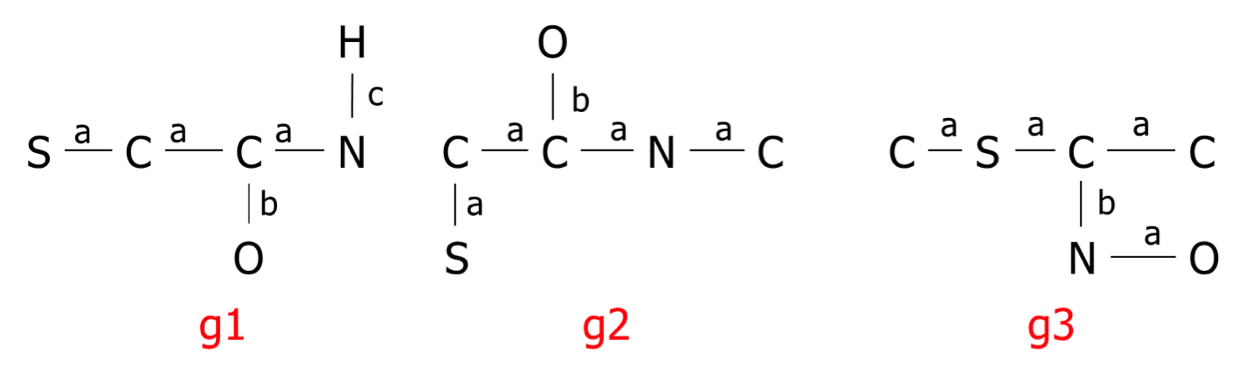
\includegraphics[scale=0.5]{gspan.png} 
				\end{center}
				gSpan is an algorithm for mining frequent graph patterns. On the course page, download the gSpan package and complete the following questions.\\
				
				\textbf{Purpose} 
				\begin{itemize}\vspace{-2mm}\setlength\itemsep{-1mm}
					\item Work on graph mining using \textit{gSpan}
					\item Learn how to utilize gSpan package by converting graph and pattern into files of correct format.
				\end{itemize}
				
				\textbf{Requirements}
				\begin{itemize}\vspace{-2mm}\setlength\itemsep{-1mm}
					\item For each question, draw all the pattern graphs as given from the gSpan algorithm. Like what we did in class, we start with a tree of empty root node and generate patterns by adding new nodes as children of the pattern tree.
				\end{itemize}
				
				Here is three molecular formulas of acids that we are interested in. Use gSpan to do the following:
				\begin{itemize}
					\item[(1)] (5', L2) Practice the algorithm \textbf{by hand} to find \textbf{ALL} patterns that appear in all three molecular structures. Draw the pattern grow tree and list the pattern and its frequency of each node. \textbf{For this question, it is fine to draw the tree by hand and take a picture of it and paste in the answer.} (\textit{Hint: the frequency is counted by the number of molecular structures it appears, not by its number of occurrences. E.g., the frequency of O-H is 3, though it appears four time.})
					\item[(2)] (5', L2) Now, use the gSpan \textbf{package} to find \textbf{ALL} patterns that appear in at least two molecules. Note that the executable binary we have is compiled on Linux. You will need to use a Linux machine (such as EWS) to run the algorithm (though you can hack a little bit to run Linux binary on Mac by emulating --- do a Google search for related results.)
					\item[(3)] (5', L2) Find the closed patterns from the result of (2). Considering that sulfuric acid is a typical inorganic acid while acetic acid is organic, what can you say that determins the acidity of organic/inorganic compound in general?
				\end{itemize}
				
				
			\end{document}